\chapter{Experiments and Evaluation}
\label{ch:evaluation}

This chapter reports the results of the experiments described in Chapter~\ref{ch:methods}
and concentrates on the results that answer the research questions.
Section~\ref{sec:eval_emotion} first establishes how well emotion can be predicted from
audio, since the pipeline depends on it. Section~\ref{sec:eval_genre} answers RQ1, whether
a soundtrack's emotional profile predicts its film's genre, and
Section~\ref{sec:eval_direct} answers RQ2b within one dataset: whether the detour through
emotion beats classifying genre directly from audio. Section~\ref{sec:eval_pergenre}
breaks this comparison down by genre. Section~\ref{sec:eval_signatures} answers RQ2a and
RQ3, which emotions relate to which genres, and Section~\ref{sec:eval_transfer} answers
RQ2b across datasets, on film music the model has never seen. Analyses that check these
results without changing them (the choice of metric, stability over seeds, the emotion
ablation, the waveform representation, all eight genres, the reproduction of the published
Blockbuster result and an error analysis) are reported in
Appendix~\ref{app:supplementary}.

Two conventions apply throughout. First, every genre score is macro-$F_1$ over films
(Section~\ref{sec:evaluation_protocol}): the predicted probabilities of a film's clips are
averaged, and the film is scored once. Where it matters for the argument, the clip-level
score of the same predictions is given beside it. Second, results come from three label
spaces that are never compared directly: the eight Eerola genres (346 clips,
42 films), the five-genre subset (329 clips, 40 films) on which the
in-domain comparisons are made, and the six genres shared with the Blockbuster dataset
(319 Eerola clips from 40 films, and 110 Blockbuster films). Every score is
therefore given with the chance floor of its own label space, either the
\emph{most-frequent} baseline or the higher \emph{base-rate random guess}
(Section~\ref{sec:fund_evaluation}).

% =============================================================================
\section{Stage 1: Emotion Regression}
\label{sec:eval_emotion}

The first stage predicts the eight emotion ratings from a frozen audio embedding with a
random forest. It is scored by $R^2$, averaged over the eight emotions, on out-of-fold
predictions of five-fold cross-validation grouped by film over all 360 rated clips
(Section~\ref{sec:evaluation_protocol}). Table~\ref{tab:waveform_stage1} ranks the six
audio representations, and Figure~\ref{fig:stage1_r2} breaks the result down by emotion.
The last column of the table expresses each score as a fraction of $R^2 = 0.897$, the
agreement between two independent listener panels (Section~\ref{subsec:rating_reliability}).

\begin{table}[tbp]
  \centering
  \caption{Emotion regression by audio representation: mean $R^2$ over the eight emotions.}
  \label{tab:waveform_stage1}
  \begin{tabular}{llrrrr}
    \toprule
    Representation & Input domain & Dim. & $R^2$ & RMSE & \% of ceiling \\
    \midrule
    CLAP             & log-mel spectrogram & 512 & 0.558 & 1.22 & 62 \\
    VGGish           & log-mel spectrogram & 128 & 0.553 & 1.23 & 62 \\
    AST              & log-mel spectrogram & 768 & 0.545 & 1.24 & 61 \\
    MusiCNN          & log-mel spectrogram & 200 & 0.512 & 1.29 & 57 \\
    Hand-crafted MIR & STFT descriptors    & 103 & 0.476 & 1.33 & 53 \\
    wav2vec 2.0      & raw waveform        & 768 & 0.299 & 1.54 & 33 \\
    \bottomrule
  \end{tabular}
\end{table}

\begin{figure}[t]
  \centering
  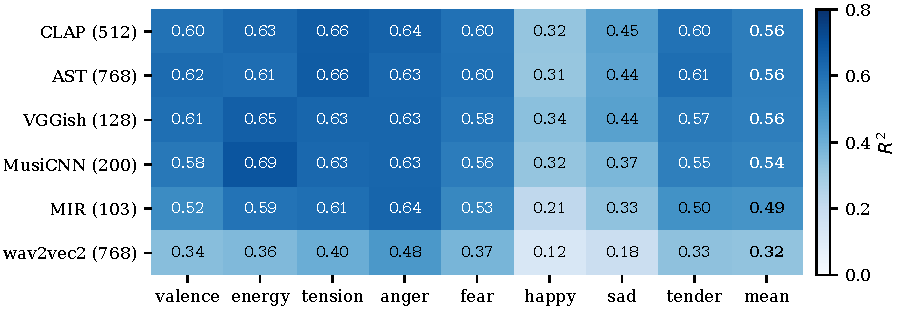
\includegraphics[width=\textwidth]{figures/stage1_r2.pdf}
  \caption{Stage~1: $R^2$ per emotion and audio representation (film-grouped cross-validation, 360 rated clips).}
  \label{fig:stage1_r2}
\end{figure}

Each cell of Figure~\ref{fig:stage1_r2} is the $R^2$ of the regressor for one emotion
(column) and one representation (row); the last column is the mean over the eight
emotions. $R^2=0$ corresponds to always predicting the mean rating.

The three general-purpose spectrogram embeddings, CLAP, VGGish and AST, cannot be told apart
($R^2$ between 0.545 and 0.558). The music-pretrained MusiCNN follows closely
(0.512), the 103 hand-crafted descriptors are clearly weaker (0.476), and the
waveform model wav2vec~2.0 recovers far less of the rating variance than any other
(0.299). The emotions also differ in difficulty. For the three strongest
representations, tension, energy and anger are the easiest ($R^2$ 0.608 to
0.661), valence and fear follow (0.559 to 0.603), and sadness
(0.428 to 0.438) and happiness (0.302 to 0.321) are clearly the
hardest. This mirrors the ``valence problem'' of music emotion recognition, where arousal
is recovered from audio more reliably than the positive--negative quality of an emotion
\citep{kim2010music,kang2025there}.

\subsection{Reliability of the Ratings and the Attainable Ceiling}
\label{subsec:rating_reliability}

The ratings that the regressor is scored against are themselves noisy. The dataset of
\citet{eerola2011comparison} allows a direct estimate: its second set re-rates clips from
the first with a different listener panel, which gives two independent measurements of
the same music on 102 matched clips. The panels agree closely (mean correlation over the
eight emotions $r=0.912$, intraclass correlation for consistency ICC(C,1) $=0.897$),
although on the three bipolar scales the second panel rated systematically higher, which
lowers absolute agreement to ICC(A,1) $=0.818$. A predictor cannot agree with a noisy
target more closely than the target agrees with an independent measurement of itself, so
the attainable $R^2$ is about 0.897. The best representations reach 62\,\% of
it. Rating noise is therefore not what limits the regressor; the limit lies in the audio
representations and the amount of training data.

% =============================================================================
\section{Genre Classification from Emotion (RQ1)}
\label{sec:eval_genre}

All genre results in this and the next two sections use $10\times5$ cross-validation
grouped by film with nested tuning of $C$. Each repeat is scored once on its pooled
out-of-fold predictions, per film, and the scores are averaged over the ten repeats, with a
95\,\% interval from a bootstrap over films.

On the five-genre subset, a classifier trained on the human emotion ratings reaches a
film-level macro-$F_1$ of 0.491 [0.411, 0.552], and the full pipeline, in which
the emotions are predicted from the VGGish embedding, reaches 0.460 [0.385, 0.514]
(Figure~\ref{fig:indomain_eerola5}). Both lie far above the most-frequent baseline
(0.168) and clearly above the base-rate random guess (0.309). Scored over clips, the same
predictions reach 0.416 and 0.405. RQ1 can therefore be answered positively: the
emotional profile of a film's soundtrack predicts its genres well above chance, although
far from perfectly. The same holds on all eight genres, where the pipeline reaches 0.349
against a random guess of 0.226 (Appendix~\ref{sec:app_eight}).

\begin{figure}[t]
  \centering
  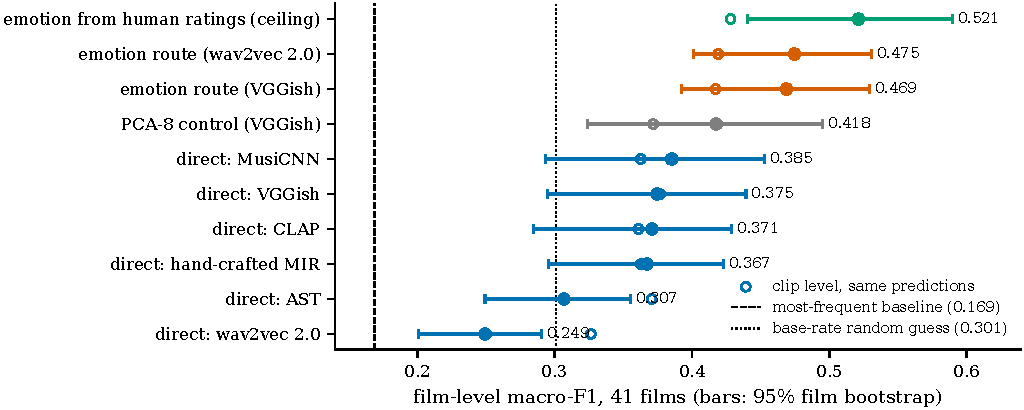
\includegraphics[width=\textwidth]{figures/indomain_eerola5.pdf}
  \caption{Genre classification on the five-genre Eerola subset: film-level macro-$F_1$ of every route with 95\,\% intervals.}
  \label{fig:indomain_eerola5}
\end{figure}

In Figure~\ref{fig:indomain_eerola5}, each filled point is the film-level macro-$F_1$,
averaged over the ten repeats, and the whiskers are 95\,\% intervals from a bootstrap over
films. The hollow marker in each row is the clip-level score of the same predictions.
Green marks the classifier on the human ratings (the ceiling of the emotion route), orange
the emotion route, blue an audio representation used directly, and grey the PCA-8
control. The dashed line is the most-frequent baseline and the dotted line the base-rate
random guess.

For the use of the pipeline, the most important comparison is between predicted and rated
emotions. At film level the ratings score 0.032 higher (difference $-0.032$ [$-0.090$,
$+0.021$]) and are ahead in all ten repeats, but the difference is not
significant ($p=0.277$); over clips the two are level ($-0.010$, $p=0.340$). Emotions
estimated from audio therefore carry most of the genre information in the ratings they were
trained on, so the pipeline needs no emotion annotation at deployment, although a better
emotion model might still gain a little.

% =============================================================================
\section{Emotion versus Direct Audio, In-domain (RQ2b)}
\label{sec:eval_direct}

Figure~\ref{fig:indomain_eerola5} also answers RQ2b within one dataset. Used directly, the
six representations reach MusiCNN 0.396, CLAP 0.390, VGGish 0.367, the hand-crafted descriptors 0.365, AST 0.318 and wav2vec~2.0 0.261. The PCA-8 control, which compresses the VGGish
embedding to eight principal components, reaches 0.390. The emotion route from the same
VGGish embedding reaches 0.460 and is ahead of all of them, by 0.065 to 0.196.
Table~\ref{tab:power_cmp} gives the comparisons that matter most for the argument; all
paired comparisons are listed in Appendix~\ref{sec:app_comparisons}.

\begin{table}[tbp]
  \centering
  \small
  \caption{The main paired comparisons on the five-genre subset (40 films).}
  \label{tab:power_cmp}
  \setlength{\tabcolsep}{4pt}
  \begin{tabular}{lrcrr@{\hspace{10pt}}rr}
    \toprule
    & \multicolumn{4}{c}{Film level} & \multicolumn{2}{c}{Clip level} \\
    \cmidrule(lr){2-5} \cmidrule(lr){6-7}
    Comparison & $\Delta$ & 95\,\% CI & $p_{\text{boot}}$ & won & $\Delta$ & $p_{\text{NB}}$ \\
    \midrule
    Emotion vs.\ VGGish (its input)     & $+0.093$ & $[-0.001,\,+0.191]$ & $0.052$ & 9 & $+0.039$ & $0.086$ \\
    Emotion vs.\ MusiCNN (best direct)  & $+0.065$ & $[-0.039,\,+0.170]$ & $0.241$ & 9 & $+0.046$ & $0.112$ \\
    Emotion vs.\ PCA-8 control          & $+0.070$ & $[-0.011,\,+0.158]$ & $0.089$ & 10 & $+0.042$ & $0.151$ \\
    Emotion vs.\ ground truth           & $-0.032$ & $[-0.090,\,+0.021]$ & $0.277$ & 0 & $-0.010$ & $0.489$ \\
    \bottomrule
  \end{tabular}
\end{table}

In Table~\ref{tab:power_cmp}, $\Delta$ is the first route minus the second with its 95\,\%
interval and $p$-value from the paired film bootstrap, and ``won'' counts the ten repeats
in which the first route scores higher. The two right-hand columns score the same
predictions over clips with the Nadeau--Bengio corrected $t$-test, which needs one score per
test fold and therefore cannot be computed per film. Bold marks $p<0.05$.

Three results stand out. First, the emotion route is ahead of the VGGish embedding it is
computed from by $+0.093$, in 9 of ten repeats, and ahead of every other direct
representation as well. Whether these leads are significant depends on the comparison and
on the unit of scoring. At film level the film bootstrap finds the lead significant against
AST, the hand-crafted descriptors and wav2vec~2.0, but not against VGGish ($p=0.052$), CLAP ($p=0.156$) and MusiCNN ($p=0.241$). Over clips, where the leads are smaller
(0.037 to 0.049), the same bootstrap finds it significant against
VGGish, CLAP, MusiCNN, the hand-crafted descriptors and wav2vec~2.0 but not against AST ($p=0.106$), and the stricter Nadeau--Bengio test,
whose attainable $p$-value lies above 0.05 on this dataset, only against wav2vec~2.0
(Appendix~\ref{sec:app_comparisons}).
Second, compression alone explains part of the film-level gain. The PCA-8 control is ahead
of VGGish by $+0.023$ ($p=0.488$, but in 7 of ten repeats and under every seed), and
the emotion route's lead over the control, $+0.070$, is not significant ($p=0.089$). Over
clips the control is level with VGGish and the emotion route is ahead of it ($+0.042$,
$p=0.020$). Third, part of the advantage is an operating-point effect. With a decision
threshold tuned per genre on the training folds, the routes converge over clips (0.420
to 0.433; Appendix~\ref{sec:eval_robustness}). The in-domain answer to RQ2b is
therefore that the emotion route is consistently ahead of direct audio at the default
threshold, in nearly every repeat and under every seed, but that the size of its lead over
the strongest direct representations is not established on 40 films.

These numbers are stable. Re-running the entire protocol under five master seeds moves the
ten-repeat mean of the emotion route by at most 0.019 (from 0.460 to
0.481), and its lead over VGGish stays positive under every seed ($+0.076$ to
$+0.132$). The main source of uncertainty is which films the dataset happens to
contain (bootstrap standard error 0.027 to 0.038), which only more films could reduce
(Appendix~\ref{sec:eval_robustness}).

% =============================================================================
\section{Results per Genre}
\label{sec:eval_pergenre}

Macro-$F_1$ averages five very different genres. Figure~\ref{fig:per_genre} shows the
film-level $F_1$ of every route for each genre, and Table~\ref{tab:per_genre} adds
precision and recall for the emotion route and for VGGish, the embedding it is computed
from.

\begin{figure}[t]
  \centering
  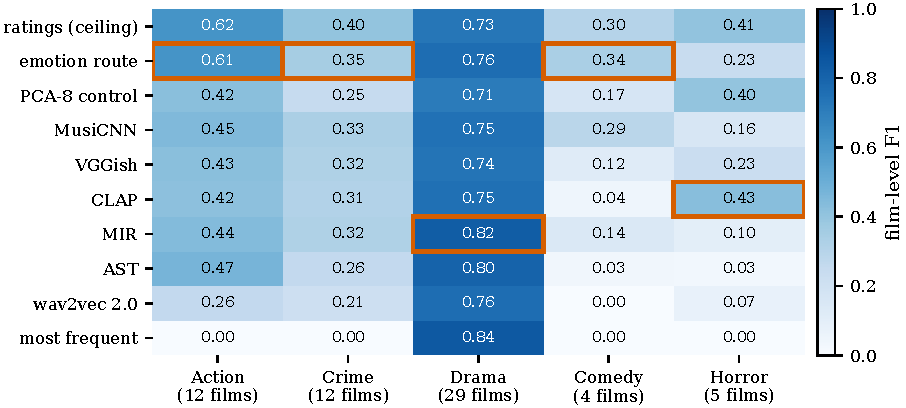
\includegraphics[width=\textwidth]{figures/per_genre.pdf}
  \caption{Film-level $F_1$ per genre and route on the five-genre subset.}
  \label{fig:per_genre}
\end{figure}

In Figure~\ref{fig:per_genre}, each cell is a route's $F_1$ for one genre, averaged over
the ten repeats; the number of films with the genre is given under its name. The box marks
the best route for each genre among the emotion route, the PCA-8 control and the six
direct representations; the ratings (the ceiling) and the most-frequent baseline are shown
for reference but not boxed.

\begin{table}[tbp]
  \centering
  \small
  \caption{Precision, recall and $F_1$ per genre at film level: best route, emotion route and VGGish.}
  \label{tab:per_genre}
  \setlength{\tabcolsep}{4pt}
  \begin{tabular}{lrlrrrrrr}
    \toprule
    & & & \multicolumn{3}{c}{Emotion route} & \multicolumn{3}{c}{VGGish direct} \\
    \cmidrule(lr){4-6} \cmidrule(lr){7-9}
    Genre & Films & Best route ($F_1$) & Prec. & Rec. & $F_1$ & Prec. & Rec. & $F_1$ \\
    \midrule
    Action   & 12 & Emotion (0.61) & 0.52 & 0.76 & \textbf{0.61} & 0.39 & 0.47 & 0.43 \\
    Crime    & 12 & Emotion (0.35) & 0.28 & 0.47 & \textbf{0.35} & 0.29 & 0.37 & 0.32 \\
    Drama    & 29 & MIR (0.82) & 0.87 & 0.68 & \textbf{0.76} & 0.79 & 0.69 & 0.74 \\
    Comedy   & 4 & Emotion (0.34) & 0.22 & 0.78 & \textbf{0.34} & 0.12 & 0.12 & 0.12 \\
    Horror   & 5 & CLAP (0.43) & 0.15 & 0.50 & \textbf{0.23} & 0.21 & 0.26 & 0.23 \\
    \bottomrule
  \end{tabular}
\end{table}

In Table~\ref{tab:per_genre}, all values are film-level and averaged over the ten repeats;
``Best route'' is the route with the highest $F_1$ for the genre, as boxed in
Figure~\ref{fig:per_genre}.

The emotion route is the best route for Action, Crime and Comedy. For Drama the best route is the hand-crafted MIR features (0.82 against 0.76 for the emotion route), and for Horror it is CLAP (0.43 against 0.23). Drama, the
genre of 29 of the 40 films, is predicted well by every route, including the
most-frequent baseline, and so separates the routes least. The largest difference lies in
Comedy (4 films). Its VGGish probabilities rarely average above one half over a
film's clips, so VGGish seldom predicts it (recall 0.12), whereas the emotion route
finds most Comedy films (recall 0.78) at a low precision (0.22). Horror
(5 films) is the exception: although fear defines it, the emotion route predicts
it for too many films (precision 0.15 at a recall of 0.50) and is no better
than VGGish there (0.23 against 0.23). Averaged over the five genres, the
emotion route has a recall of 0.64 against 0.38 for VGGish, at a precision of 0.41
against 0.36. Its advantage is therefore mainly that it finds the rare genres, at the
price of more false positives, which is the same recall-driven pattern as the
operating-point effect of Section~\ref{sec:eval_direct}. With only four or five films behind the two rarest
genres, their $F_1$ values move by about 0.2 when a single film changes, and the per-genre
comparison should be read as a description, not as a test.

% =============================================================================
\section{Emotional Signatures of Genres (RQ2a, RQ3)}
\label{sec:eval_signatures}

RQ2a and RQ3 concern the content of the relationship rather than its predictive strength.
They are answered with Cohen's $d$ (Section~\ref{sec:fund_evaluation}), computed for each
emotion rating between the clips of a genre and all other clips.
Table~\ref{tab:emotion_genre_signatures} summarises the dominant signature of each of the
eight Eerola genres; a positive $d$ means that the emotion is elevated in the genre.

\begin{table}[tbp]
  \centering
  \caption{Dominant emotional signature (Cohen's $d$) of each of the eight Eerola genres.}
  \label{tab:emotion_genre_signatures}
  \begin{tabular}{llr}
    \toprule
    Genre       & Dominant emotion (direction) & Cohen's $d$ \\
    \midrule
    Horror      & fear (high)            & $+0.75$ \\
    Biography   & happiness (high)       & $+0.67$ \\
    Comedy      & fear (low)             & $-0.61$ \\
    Drama       & valence (high)         & $+0.57$ \\
    Documentary & anger (low)            & $-0.51$ \\
    Action      & happiness (low)        & $-0.50$ \\
    Crime       & fear (high)            & $+0.40$ \\
    Adventure   & none with $|d|>0.25$   & -- \\
    \bottomrule
  \end{tabular}
\end{table}

Fear is the strongest single discriminator. It separates the threat-oriented genres
(Horror, $d=+0.75$, the strongest genre--emotion association in the dataset; Crime,
$+0.40$) from the light-hearted ones (Comedy, $-0.61$). Valence forms a second axis,
separating the positively toned genres (Drama, $+0.57$; Comedy) from the negatively toned
ones (Horror, $-0.63$; Action). Each of these genres thus has an affective fingerprint that
agrees with film-scoring convention: Horror is defined by fear, Comedy by the absence of
fear together with positive valence, Drama by elevated valence, and Action by high tension
without happiness. The signatures of Biography and Documentary are also strong, but they
rest on very few films. Adventure has no signature: no emotion exceeds $|d|=0.25$, as the
genre co-occurs with several others and shares their affective palette. This mirrors the
asymmetry reported by \citet{austin2010characterization}: genres with a conventional
affective identity are recoverable from the music, while genres defined by narrative or
setting are not. For RQ2a, emotions relate to most genres in a systematic and readable
way; for RQ3, fear is the most discriminating emotion overall, followed by valence.

\subsection{Do the Signatures Replicate?}
\label{subsec:signature_replication}

The signatures were derived from human ratings on one dataset. Whether they describe film
music or only that dataset can be tested on the second one. The Eerola-trained emotion
regressor predicts the eight emotions for each of the 4664 Blockbuster cues, and the same
effect sizes are recomputed there for the six shared genres. No emotion annotation of
Blockbuster exists or is used, so any agreement comes from transfer and not from fitting.
Figure~\ref{fig:signatures} shows the two matrices side by side.

\begin{figure}[t]
  \centering
  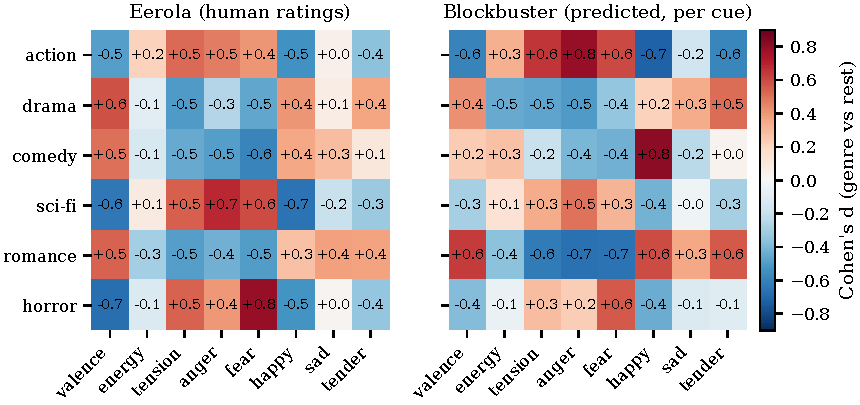
\includegraphics[width=\textwidth]{figures/signatures.pdf}
  \caption{Emotional signatures (Cohen's $d$) of the six shared genres on Eerola (left) and Blockbuster (right).}
  \label{fig:signatures}
\end{figure}

Each cell of Figure~\ref{fig:signatures} is Cohen's $d$ of one emotion for one genre
against all other items; red marks an emotion elevated in the genre, blue a suppressed one.
The Eerola matrix is computed from the human ratings, the Blockbuster matrix from the
emotions predicted for each cue.

The signatures replicate. Across all 48 genre--emotion cells, the Eerola effect sizes and
the film-level Blockbuster ones correlate at $r=0.836$, and 92\,\% of the signs
agree. Horror is defined by fear in both datasets. The replication is closest for Romance,
Sci-Fi, Action and Horror and weakest for Comedy, whose strongest emotion changes from fear
to happiness. The absolute effect sizes do not transfer: averaging some 39 cues per film
inflates $d$, and measured per cue the values are of the same order as on Eerola. The
structure of the emotion--genre relationship therefore generalises beyond its own
dataset, although, since the Blockbuster emotions are predicted by a model trained on the
Eerola panel, the replication cannot show independence from that panel.

% =============================================================================
\section{Cross-Dataset Transfer (RQ2b under domain shift)}
\label{sec:eval_transfer}

The results so far are cross-validated within one dataset. They show that a representation
carries genre information, but not that this information is a property of film music
rather than of one collection of films. The experiments in this section therefore train on
one dataset and test on the other, in the six-genre space shared with the Blockbuster
dataset of \citet{ma2021computational} (Section~\ref{subsec:genre_labels}). VGGish is the
only representation available on both (Section~\ref{subsec:methods_blockbuster}). Since a
Blockbuster row is a film, every score in this section is a film-level score, as in the
in-domain sections. On the 110 Blockbuster films the base-rate random guess reaches
0.292 and the plurality baseline 0.193; on the 40 Eerola films of the shared
space the random guess reaches 0.240.

\paragraph{No film occurs in both datasets.} A transfer result would be inflated if the
same film were in the training and the test data. This was checked against the IMDb
identifiers of all films: none of the 42 Eerola films occurs among the 110
Blockbuster films, and no titles match. The Eerola films were all released before 2011,
the Blockbuster films between 2014 and 2019. The two datasets share composers, however
(for example, Danny Elfman scored \emph{Batman} in Eerola and \emph{Justice League} in
Blockbuster, which quotes his Batman theme), so some stylistic similarity across the split
remains possible; it is not a shared film. A related problem was found inside the Eerola
dataset and corrected before the results reported here: one film appeared under two
spellings of its title, so that grouping by film treated it as two films and could place
its clips on both sides of a split. All Eerola experiments were re-run with the two
spellings merged, which gives the 42 films (eight genres) and 40 films (five
genres) used throughout.

\subsection{Blockbuster in-domain}

A transfer score needs an in-domain reference on the target. The simple pipeline of this
thesis first reproduces the published result on Blockbuster: under the leave-one-film-out
protocol of \citet{ma2021computational} it reaches macro-$F_1$ 0.620, within the 0.61 to
0.65 they report for their VGGish models (Appendix~\ref{sec:app_blockbuster}).
Figure~\ref{fig:blockbuster_cv} shows the same dataset under the repeated protocol used for
Eerola ($10\times5$ cross-validation over films).

\begin{figure}[t]
  \centering
  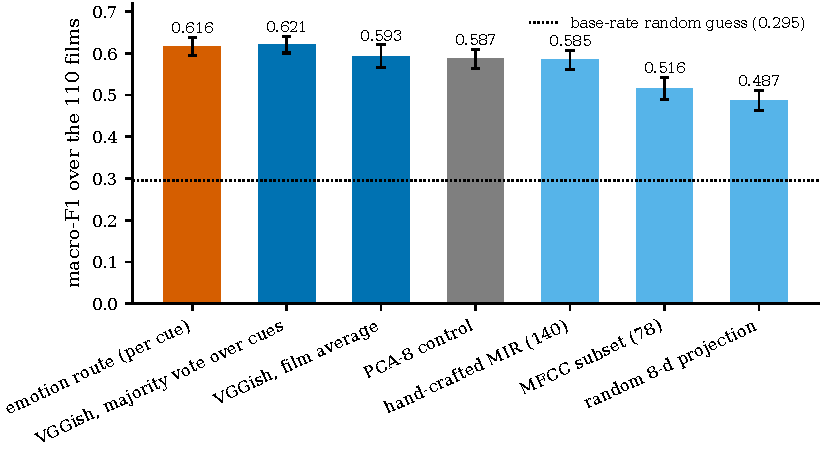
\includegraphics[width=\textwidth]{figures/blockbuster_cv.pdf}
  \caption{Blockbuster in-domain: macro-$F_1$ over the 110 films under $10\times5$ cross-validation.}
  \label{fig:blockbuster_cv}
\end{figure}

In Figure~\ref{fig:blockbuster_cv}, each bar is the mean over the 50 folds and the error
bar the standard deviation of the ten repeat means; the dotted line is the base-rate
random guess (0.295). The emotion route is applied per cue and its emotions averaged per
film; ``majority vote over cues'' classifies each cue and lets the cues vote, as in the
best model of \citet{ma2021computational}.

In-domain on Blockbuster, the emotion route (0.616 $\pm$ 0.022) is level with
direct audio. It is nominally ahead of the film-average VGGish embedding (0.593;
$+0.023$, Nadeau--Bengio $p=0.536$) and slightly behind VGGish with a majority vote
over cues (0.621), and none of these differences is significant. The PCA-8 control
(0.587) is a serious baseline here, well ahead of a random eight-dimensional projection
of the same embedding (0.487). The hand-crafted MIR features (0.585) are level with
VGGish ($+0.009$, $p=0.787$).

\subsection{Zero-Shot Transfer}
\label{sec:zero_shot}

In the zero-shot experiment every model is fitted on the Eerola dataset alone and used to
predict the genres of all 110 Blockbuster films; no Blockbuster label takes part in
training. The emotion classifier is trained on out-of-fold predicted emotions, so that it
sees the same kind of noisy input it meets at test time. A single train--test split has no
fold structure, so uncertainty comes from a paired bootstrap over the 110 target films. The
feature scaler is the one fitted on the source dataset (the strict regime), which is the
conservative choice because the direct baseline scores higher under it.
Figure~\ref{fig:zero_shot} shows the result and Table~\ref{tab:zero_shot} gives precision
and recall.

\begin{figure}[t]
  \centering
  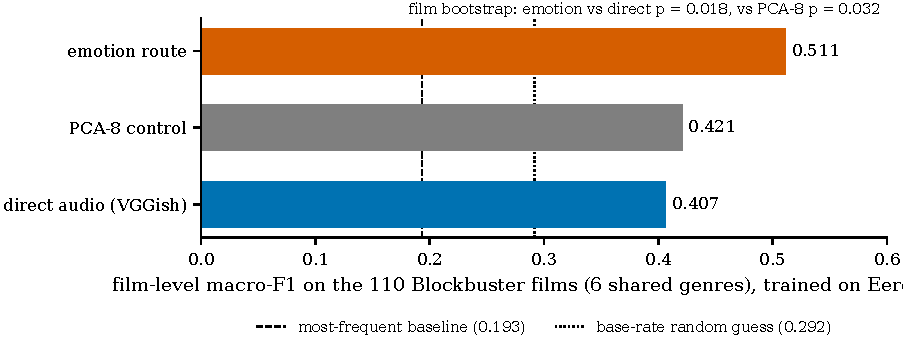
\includegraphics[width=\textwidth]{figures/zero_shot.pdf}
  \caption{Zero-shot transfer from Eerola to the 110 Blockbuster films (six shared genres, strict regime).}
  \label{fig:zero_shot}
\end{figure}

In Figure~\ref{fig:zero_shot}, the dashed line is the plurality baseline and the dotted line
the base-rate random guess; the $p$-values are paired bootstraps over the 110 films.

\begin{table}[tbp]
  \centering
  \caption{Zero-shot transfer from Eerola to the 110 Blockbuster films (strict regime).}
  \label{tab:zero_shot}
  \begin{tabular}{lrrr}
    \toprule
    Approach (trained on Eerola only) & Prec. & Rec. & $F_1$ \\
    \midrule
    VGGish $\rightarrow$ predicted emotion (11), per cue            & 0.480 & 0.651 & \textbf{0.508} \\
    PCA-8 (VGGish) $\rightarrow$ genre (control)                    & 0.539 & 0.459 & 0.417 \\
    VGGish-128 $\rightarrow$ genre (direct)                         & 0.705 & 0.435 & 0.403 \\
    Random guess                                                    & 0.294 & 0.293 & 0.292 \\
    \midrule
    \emph{In-domain reference (trained on Blockbuster)}             & \emph{0.569} & \emph{0.705} & \emph{0.620} \\
    \bottomrule
  \end{tabular}
\end{table}

Genre information transfers between the datasets. The emotion route reaches 0.508
against a random-guess floor of 0.292, about 82\,\% of the 0.620 obtained with
in-domain training, although each training row is a clip of about 17 seconds and the
test items are whole films. The central result for RQ2b is that the emotion route
transfers better than the representation it is derived from: it exceeds direct VGGish
(0.403) by $+0.106$ [$+0.021$, $+0.184$] ($p=0.013$), and the PCA-8 control
(0.417) by $+0.093$ [$+0.013$, $+0.171$] ($p=0.027$), whereas compressing the
embedding to eight principal components gains only $+0.013$ over the raw features
($p=0.737$). Under the alternative scaling regime the lead over direct VGGish is
$+0.118$ ($p=0.001$). The lead is partly recall-driven: the emotion route finds more of
the true genres (0.651 against 0.435) at lower precision (0.480 against
0.705). In this transfer it makes little difference whether the emotions are predicted
per cue or once from the film-average embedding (0.508 against 0.502); in-domain on
Blockbuster the per-cue prediction is clearly better (Appendix~\ref{sec:app_blockbuster}).

\subsection{Transfer in Every Direction}

Two further designs complete the picture (Figure~\ref{fig:cross_dataset}). In the reverse
direction, the genre classifier is trained on all Blockbuster films and tested on the
Eerola films; the emotion regressor is fitted on the Eerola training folds, and the
held-out Eerola films touch neither fit. In the pooled design both datasets are in the
training set and cross-validation runs over both.

\begin{figure}[t]
  \centering
  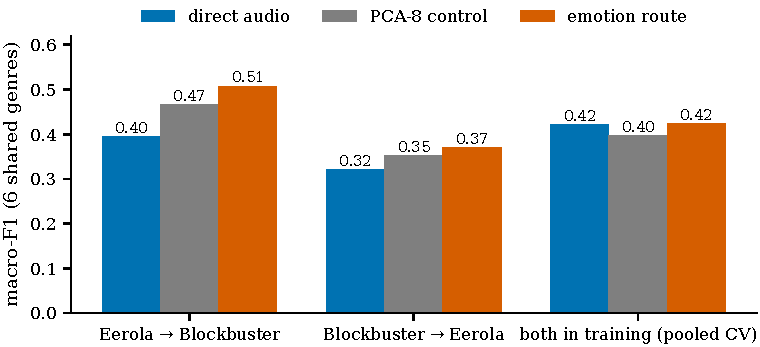
\includegraphics[width=\textwidth]{figures/cross_dataset.pdf}
  \caption{Film-level macro-$F_1$ for the three cross-dataset designs (six shared genres, VGGish).}
  \label{fig:cross_dataset}
\end{figure}

In Figure~\ref{fig:cross_dataset}, the left group is trained on Eerola and tested on
Blockbuster, the middle group trained on Blockbuster and tested on Eerola, and the right
group cross-validated with both datasets in training. The error bars are the bootstrap
standard deviation over the test films for the two transfer directions and the standard
deviation of the five repeat means for the pooled design. The left group comes from a
re-implementation in which the emotion regressor is trained on all 360 rated clips, so it
differs slightly from Figure~\ref{fig:zero_shot}.

The emotion route is ahead of direct VGGish in both transfer directions, but significantly
only from Eerola to Blockbuster (0.503 against 0.383, $+0.121$, $p=0.007$). From
Blockbuster to Eerola it reaches 0.458 against 0.364 ($+0.089$ [$-0.017$, $+0.206$],
$p=0.102$), against a random-guess floor of 0.240. Over clips, with whole films
resampled, the reverse difference is $+0.027$ ($p=0.069$); an earlier version of this
analysis resampled clips, which are not independent, and reported it as significant. When
both datasets are in the
training set the advantage disappears: per film, the emotion route (0.531) and direct
VGGish (0.543) are level ($-0.011$, Nadeau--Bengio $p=0.688$). The pooled design also
shows where each route is strong. On the Eerola films of the pooled test folds the emotion
route leads (0.528 against 0.410), and on the Blockbuster films direct audio does
(0.579 against 0.568).

The comparison with the PCA-8 control is less robust than the one with direct audio. The
two implementations of the Eerola-to-Blockbuster direction differ in one legitimate choice
(the emotion regressor is trained on the 319 clips of the shared space in the zero-shot
experiment and on all 360 rated clips in the re-implementation). The emotion route is
stable between them (0.508 and 0.503), but the PCA-8 control moves from 0.417 to
0.457, and the emotion route's lead over it is no longer significant ($+0.049$,
$p=0.239$; reverse direction $+0.070$, $p=0.158$). Single-split scores move by a few
hundredths with such choices, so the conclusion rests on the intervals rather than on the
third decimal.

% =============================================================================
\section{Summary of Findings}
\label{sec:eval_summary}

\emph{RQ1.} The emotional profile of a soundtrack predicts its film's genres well above
chance. On the five-genre subset the pipeline reaches a film-level macro-$F_1$ of 0.460,
against 0.309 for a random guess, and the human ratings reach 0.491. The emotion
regression it rests on reaches about 62\,\% of the $R^2$ that two listener
panels allow.

\emph{RQ2a and RQ3.} Most genres carry a readable affective signature. Fear is the
strongest discriminator and valence the second axis; Adventure has no signature. The
signatures replicate on the Blockbuster dataset from predicted emotions ($r=0.836$).

\emph{RQ2b in-domain.} The emotion route is ahead of every direct audio representation
(by $+0.093$ over VGGish, its own input) and of the PCA-8 control in nearly every repeat and
under every seed, and it is the best route for Action, Crime and Comedy. Its lead is significant
against the weaker direct representations, but not established against the stronger ones
or against the PCA-8 control; part of the gain comes from compression, and with per-genre
thresholds the routes converge.

\emph{RQ2b across datasets.} Trained on Eerola and tested on the 110 Blockbuster films,
the emotion route beats direct VGGish clearly (0.508 against 0.403, $p=0.013$). The
reverse direction agrees in sign without being significant, and when both datasets are in
training the routes are level. No film occurs in both datasets.

The main limitation is the size of the Eerola dataset: 40 films, two of the five
genres with four or five films each, and a film-sampling error of the same order as the
effects being measured. The results also give two different pictures. The emotion route
is clearly ahead where the genre classifier is trained on the small Eerola dataset, and
level where it is trained on the larger Blockbuster dataset or on both.
